% Definimos el estilo del documento
\documentclass[12pt,a4paper,spanish]{book}

\usepackage[utf8]{inputenc}
\usepackage[spanish]{babel}
\usepackage{ amssymb }
\usepackage{ amsmath }
\usepackage{ amsthm }
\usepackage{ wasysym }
\usepackage{ verbatim }

\usepackage{ appendix }
\renewcommand{\appendixname}{Apéndices}
\renewcommand{\appendixtocname}{Apéndices}
\renewcommand{\appendixpagename}{Apéndices}
 
%\usepackage[dvips]{graphicx}
%\DeclareGraphicsExtensions{.pdf,.png,.jpg}

\usepackage{graphicx}

\usepackage{hyperref}
\hypersetup{colorlinks=false}

\usepackage{proof}

\newtheorem{definicion}{Definición}

%Empieza el documento
\begin{document}

% Definimos titulo, autor, fecha.
\title{FROB: Un lenguaje de programación funcional reactivo para robots con bajas capacidades de cómputo}
\author{Guillermo Pacheco}
\date{\today}

% Generamos titulo e indice de contenidos
\maketitle


% Resumen
\chapter*{Resumen}
\addcontentsline{toc}{chapter}{Resumen}
\markboth{RESUMEN}{RESUMEN}


El proyecto consiste en la creación de un lenguaje de programación
para robots, cuyas capacidades de cómputo son limitadas.
Para esto se escogió el paradigma de Programación Funcional Reactiva
(\emph{FRP}) el cual permite expresar naturalmente reacciones a
valores que varían en función del tiempo.

El objetivo es utilizarlo con fines educativos,
por lo tanto debe ser simple y fácil de usar por usuarios
inexpertos, no familiarizados con la electrónica ni la informática.

Para resolver el problema, se dividió en dos etapas.

La primera consiste en la implementación de
un compilador que traduce el lenguaje cuyo nivel es alto a
un lenguaje de bajo nivel (\emph{Bytecode}) más simple e interpretable.

La segunda etapa consiste en implementar una máquina virtual, que
sea capaz de interpretar el lenguaje de bajo nivel.
Por cada plataforma objetivo, es posible realizar una implementación de
la máquina, lo que permite ejecutar los mismos
programas en alto nivel, en diferentes plataformas.

El diseño de la máquina consiste de un núcleo común capaz de interpretar
instrucciones, y módulos bien definidos de
entrada/salida los cuáles varían de una plataforma a otra.
Ésto permite mayor portabilidad y extensibilidad.

Debe ser posible ejecutar programas en dicho lenguaje dentro de plataformas
de hardware reducido.
Considerando ésto, el lenguaje de programación elegido para la
implementación de la máquina virtual es C/C++.

De esta forma se implementó un lenguaje reactivo con las
características deseadas, y una implementación modelo de una máquina
virtual que permite
su ejecución en una arquitectura objetivo deseada.
La misma es fácil de mantener, portable y cuenta con suficiente
flexibilidad para ser extendida.



% Indice general
\cleardoublepage
\addcontentsline{toc}{chapter}{Índice general} % para que aparezca en el indice de contenidos
\tableofcontents

% Indice de figuras
\cleardoublepage
\addcontentsline{toc}{chapter}{Índice de figuras} % para que aparezca en el indice de contenidos
\listoffigures

% indice de tablas
\cleardoublepage
\addcontentsline{toc}{chapter}{Índice de tablas} % para que aparezca en el indice de contenidos
\listoftables


\chapter{Introducción}
En este capítulo se realiza una introducción a la Lógica Temporal Lineal, como una extensión de Lógica 
 Proposicional para poder expresar propiedades en sistemas reactivos.
Con esta finalidad, este lenguaje fue introducido por Pnueli en \cite{pnueli}.

La Lógica Lineal Temporal permite expresar propiedades sobre los sistemas en cuestón,
 ya que se agregan operadores que hacen referencia al tiempo y permite representar los distintos estados
 en distintos momentos durante la ejecución del sistema.


\chapter{Programación Funcional Reactiva}




\section{Programación Funcional Reactiva}

Acá voy a hablar de programación funcional reactiva.

Tradicionalmente los programas son formados a partir de
una secuencia de acciones imperativas. Los programas
reactivos suelen formarse por eventos y código iterativo
que se corre cuando un evento ocurre.

Dicho código iterativo suele hacer referencia y manipular
variables compartidas con diferentes rutinas. Ésto lleva a que
como un valor puede ser manipulado desde diferentes lugares,
puedan producirse problemas de concurrencia y algunos valores
pueden quedar en un estado inconsistente.

En el paradigma FRP no existen valores compartidos, sinó que
dichos valores dependientes del tiempo, tienen una representación
llamada Comportamiento y la única forma de modificarlos, es
a partir de como fueron definidos.

 

\begin{definicion}
Comportamientos (Behaviours).\\
Un comportamiento es un valor contínuo que depende del paso del tiempo.
Los comportamientos se pueden definir, combinar, pasarlos como
argumentos a funciones, retornarlos.
Un comportamiento puede ser un valor constante, el tiempo mismo (un reloj),
o puede formarse combinando otros comportamientos, por ejemplo secuencialmente
o paralelamente.
\end{definicion}

\begin{definicion}
Eventos (Streams).\\
Son valores discretos dependientes del tiempo, que forman
una secuencia finita o infinita de ocurrencias. Cada ocurrencia
está formada por el valor y el instante de tiempo.
\end{definicion}

La principal diferencia entre Comportamientos y Eventos, es que los
comportamientos son valores contínuos y los eventos son discretos.

Los comportamientos representan cualquier valor en función del tiempo,
por ejemplo:
\begin{itemize}
\item \textit{entrada} sensor de distancia, temperatura, video
\item \textit{salida} velocidad, voltaje
\item \textit{valores} intermedios calculados
\end{itemize}

Las operaciones que se pueden realizar sobre los comportamientos incluyen:
\begin{itemize}
\item \textit{Operaciones genéricas} Aritmética, integración, diferenciación
\item \textit{Operaciones específicas de un dominio} como escalar video, aplicar filtros, detección de patrones.
\end{itemize}

Los eventos pueden ser sensores específicos de un dominio, por ejemplo un
botón, un click, una interrupción o mensaje asincrónico.
También puede ser generado a partir de valores de un comportamiento,
como ser \emph{Temperatura alta}, \emph{Batería baja}.

Las operaciones que se pueden realizar sobre los eventos incluyen:
\begin{itemize}
\item fmap, filter
\item Modificar un \emph{Comportamiento} reactivo
\end{itemize}


\section{Ejemplo}

Para entender un poco más las ideas de Comportamiento y Evento, se puede
plantear el siguiente ejemplo.

  En una cuenta de un banco, el saldo se puede definir
como un comportamiento, el cuál solo se modifica cuando ocurre
un movimiento.
  Un movimiento puede ser depositar dinero o extraer
dinero de la cuenta.
  Un dato importante a ver, es que no es posible asignar un valor
sin que sea por medio de su propia definición, por lo que nadie
podría realizar la asignación $saldo = 1000000$.
  La misma operación sería posible creando un movimiento, el cuál
afectaría al saldo.

  Usaremos la notación $<nombre> :: Event <tipo>$ para definir
eventos y la notación $<nombre> :: Behaviour <tipo>$ para
definir comportamientos.

\begin{verbatim}
movimiento :: Event Number
movimiento = read(0)

saldo :: Behaviour Number
saldo = movimiento

alert :: Event Bool
alert = saldo > 1000

on alert:
  write(0, 'El saldo es mayor a 1000')

\end{verbatim}

Un comportamiento, solo se modifica cuando cambian sus componentes,





%state = State(state, [input])
%Output(state)


%\chapter{Autómatas de Büchi}
%Los autómatas regulares fueron introducidos por Huffman \cite{huffman} como
 herramientas para reconocer palabras de largo finito.
Pero para representar las ejecuciones de un sistema se necesita trabajar con palabras de largo infinito.
Para esto Büchi introdujo el concepto de Autómatas de Büchi (NBA) \cite{buchi}.
Estos son una variante de los autómatas
 regulares utilizados para reconocer palabras de largo infinito.

%Para verificar si un sistema $TS$ dado satisface una determinada propiedad se trabaja con el autómata de
% Büchi $\mathcal{A}$, que representa los "bad traces" de la propiedad ($\mathcal{A}$ reconoce el complemento
% de la propiedad a verificar). Se realiza el producto entre $\mathcal{A}$ y $TS$ y mediante un análisis del
% grafo se determina si $TS \models P$.


\section{Lenguajes \textit{omega}-regulares}
Llamamos lenguajes regulares a los lenguajes que se pueden representar mediante expresiones regulares.
Las palabras de estos lenguajes tienen largo finito.
 %, es decir secuencias de símbolos de largo finito.
 En cambio si queremos tratar con palabras de largo infinito necesitaremos una clase distinta de
 lenguajes, asociados con una clase distinta de expresiones. Esta nueva clase de lenguajes se denomina
 lenguajes \textit{omega}-regulares.
 
%Una palabra infinita sobre el alfabeto $\Sigma$ es una secuencia de símbolos pertenecientes a $\Sigma$.
Utilizaremos la letra griega $\omega$ (\textit{omega}) para denotar la repetición infinita,
 por ejemplo $a^\omega$ es la palabra
 infinita que contiene sólo símbolos $a$.\footnote{Notar que $a^*$ representa un lenguaje, es el conjunto de todas las palabras finitas que contienen únicamente el símbolo $a$, mientras que $a^\omega$ representa
 solamente una palabra.}
 
Llamamos $\Sigma^\omega$ al conjunto de todas las palabras infinitas sobre $\Sigma$.
 Cualquier subconjunto de $\Sigma^\omega$ es un lenguaje de palabras infinitas.

\begin{definicion}
Expresión $\omega$-regular.\\
Una expresión $\omega$-regular $G$ sobre el alfabeto $\Sigma$ tiene la siguiente forma
\[ G = E_1.F_1^\omega + ... + E_n.F_n^\omega \]
donde $n \geq 1$ y $E_1, ..., E_n, F_1, ..., F_n$ son expresiones regulares sobre $\Sigma$ tales que
 $\varepsilon \not\in L(F_i)$, siendo $L(F_i)$ el lenguaje representado por la expresión regular $F_i$.
\end{definicion}

Un lenguaje $\omega$-regular, análogamente a los regulares, es un lenguaje que se puede representar
mediante una expresión $\omega$-regular.


 
 
\paragraph{Ejemplo.}
Considerando el NBA de la figura \ref{fig:nba} sobre el alfabeto $\{ A, B, C \}$.\\

\begin{figure}[hbtp]
\begin{center}
\caption{Ejemplo de Autómata de Büchi}
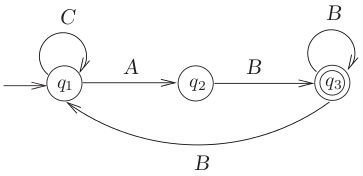
\includegraphics[width=0.7\textwidth]{buchi/imagenes/ejemplo4_28.png}
\label{fig:nba}
\end{center}
\end{figure}

El lenguaje aceptado por el NBA está dado por la expresión regular
\[ C^*AB(B^+ + BC^*AB)^\omega \]
 
\section{Autómata de Büchi Generalizado}
En este trabajo se utiliza una variante de los NBA, el Autómata de Buchi Generalizado (GNBA).
La estructura de los GNBAs es muy similar a la de los NBAs, varía sólo en el conjunto de aceptación.
En lugar de este contiene un conjunto F cuyos elementos son los conjuntos de aceptación $F_i$.
El criterio de aceptación en estos autómatas es visitar infinitas veces todos los conjuntos de
 aceptación $F_i$.

\begin{definicion}
Autómatas de Büchi Generalizado.\\
Los Autómatas de Büchi Generalizado (GNBA) consisten en una tupla $\mathcal{G} = (\text{Q}, \Sigma, \delta, \text{Q}_0, \mathcal{F})$, donde: $\text{Q}$, $\Sigma$, $\delta$ y $\text{Q}_0$ se definen
igual que en los NBA mientras que $\mathcal{F} \subseteq 2^Q$ es el conjunto de aceptación.
\end{definicion}

El lenguaje aceptado por un GNBA $\mathcal{G}$ consiste en todas las palabras que pasan infinitas
 veces por todos los conjuntos de aceptación.

Más formalmente, dado un GNBA $\mathcal{G} = (\text{Q}, \Sigma, \delta, \text{Q}_0, \mathcal{F})$ y
 una secuencia infinita de estados $q_0 q_1 q_2 q_3 ...$, esta es aceptada por $\mathcal{G}$ si
\[ \forall \text{F} \in \mathcal{F}, \exists \text{ infinitas } j \in \mathbb{N} \text{ tal que } q_j \in F \]

 
\paragraph{Ejemplo.}
En la figura \ref{fig:seccion_critica} se muestra un GNBA sobre el alfabeto $2^{AP}$
 donde $AP = \{ crit_1, crit_2 \}$ y los conjuntos de aceptación
 $F_1 = \{ q_1 \}$ y $F_2 = \{ q_2 \}$.

\begin{figure}[hbtp]
\begin{center}
\caption{GNBA para sección crítica}
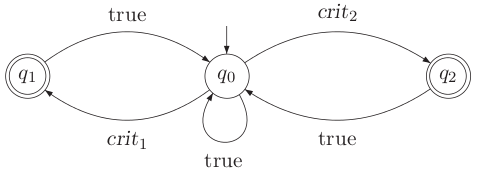
\includegraphics[width=0.7\textwidth]{buchi/imagenes/ejemplo4_53.png}
\label{fig:seccion_critica}
\end{center}
\end{figure}

El lenguaje aceptado es la propiedad que contiene todas las palabras infinitas tal que $crit_1$ y 
$crit_2$ ocurren infinitas veces.
Este GNBA representa la propiedad de que ninguno de los procesos quede infinitamente
 esperando para ingresar a la sección crítica.


%\chapter{Lógica Temporal Lineal}
%\subsection{Sintaxis de LTL}

Las fórmulas de LTL son construídas según la siguiente gramática
\[ \varphi ::= true | a | \varphi \wedge \varphi | \lnot \varphi | \bigcirc \varphi | \square \varphi | \lozenge \varphi | \varphi \cup \varphi \]

Los operadores temporales permiten establecer relaciones entre las etiquetas
 de los estados del sistema en una ejecución. Estos nuevos operadores son:

\begin{itemize}

\item $\lozenge p \longrightarrow $ eventually $p$ : 
inevitablemente en el futuro se cumplirá $p$

\item $\square p \longrightarrow $ always $p$ : 
ahora y en el futuro se cumple $p$

\item $\bigcirc p \longrightarrow $ next $p$ : 
en el siguiente paso se cumple p

\item $p \cup q \longrightarrow $ $p$ until $q$ : 
$q$ se cumplirá inevitablemente en el futuro, y mientras tanto se cumple $p$

\end{itemize}

%ejemplo 5.2 (mutua exclusión):

\paragraph{Ejemplo.}
Tomando como ejemplo el problema de mutua exclusión entre dos proceso $P_1$ y $P_2$,
 donde los procesos son modelados por tres estados:
\begin{itemize}
\item[(1)] sección no crítica
\item[(2)] espera para entrar a la sección crítica
\item[(3)] sección crítica
\end{itemize}

Sean las proposiciones $wait_i$ y $crit_i$ que representan los estados de espera y sección crítica
 respectivamente para el proceso $P_i$, se pueden representar las siguientes propiedades con LTL.
\begin{itemize}
\item $P_1$ y $P_2$ nunca acceden simultaneamente a la sección crítica
\[ \square (\neg crit_1 \vee \neg crit_2) \]
\item $P_1$ y $P_2$ acceden infinitas veces a la sección crítica
\[ (\square \lozenge crit_1) \wedge (\square \lozenge crit_2) \]
\end{itemize}


\subsection{Semántica de LTL}
La satisfacibilidad en LTL se basa en la satisfacibilidad de trazas, o más precisamente de fragmentos
de traza.
A continuación se definen los conceptos de \textit{traza} y \textit{satisfacibilidad} para
 una fórmula LTL.

\begin{definicion}
Trazas.\\
Sea un sistema de transiciones
 $\text{TS} = (\text{S}, \text{Act}, {\to}, \text{I}, \text{AP}, \text{L})$ y un fragmento de
 camino $\pi = s_0 s_1 s_2 ...$. La traza correspondiente a $\pi$ es
 $\text{Traza}(\pi) = L(s_0) L(s_1) L(s_2) ...$

Además se definen las trazas de un sistema de transiciones como:
\[ \text{Trazas}(\text{TS}) = \{ \text{Traza}(\pi) | \pi \text{ es un camino de TS} \} \]
\end{definicion}


\begin{definicion}
Satisfacibilidad en LTL para trazas.\\
Dada una traza $\sigma = A_0 A_1 A_2 ...$ y dos fórmulas LTL $\varphi$, $\psi$.
\begin{itemize}
\item $\sigma \models \textit{true}$
\item $\sigma \models a$ si y solo si $a \in A_0$
\item $\sigma \models \neg \varphi $ si y solo si $\sigma \not\models \varphi $
\item $\sigma \models \varphi \wedge \psi $ si y solo si $\sigma \models \varphi $ y $\sigma \models \psi $
\item $\sigma \models \bigcirc \varphi $ si y solo si $\sigma [1...] \models \varphi$
\item $\sigma \models \lozenge \varphi $ si y solo si $\exists j \ge 0, \sigma [j...] \models \varphi$
\item $\sigma \models \square \varphi $ si y solo si $\forall j \ge 0, \sigma [j...] \models \varphi$
\item $\sigma \models \varphi \cup \psi $ si y solo si $\exists j \ge 0, \sigma [j...] \models \psi $ y $\forall 0 \le i < j, \sigma [i...] \models \varphi $
\end{itemize}
\end{definicion}

Una vez definida la satisfacibilidad para trazas, se define la satisfacibilidad
 para un sistema de transiciones.
 
\begin{definicion}
Satisfacibilidad en LTL para un sistema de trasiciones.\\
Dado un sistema se transiciones $TS = (S, Act, \rightarrow, I, AP, L)$ y una fórmula LTL $\varphi$.

La relación de satisfacibilidad para un sistema de transiciones se define como 
\[ \text{TS} \models \varphi \text{ si y sólo si } \sigma \models \varphi, \forall \sigma \in \text{Trazas} (\text{TS}) \]
\end{definicion}







\subsection{Propiedades}
Las siguientes propiedades son necesarias para poder expresar cualquier fórmula de LTL utilizando
 un conjunto reducido de operadores ($true, \lnot, \land, \bigcirc, \cup$).

\begin{itemize}
\item $p \lor q = \lnot (\lnot p \land \lnot q)$
\item $p \rightarrow q = \lnot (p \land \lnot q)$
\item $p \leftrightarrow q = \lnot (p \land \lnot q) \land \lnot (\lnot p \land q)$
\item $\lozenge p = true \cup p$
\item $\square p = \lnot (true \cup \lnot p)$
\end{itemize}


\begin{definicion}
Conjunto funcionalmente completo de conectivos.\\
Sea un conjunto de conectivos $C$. Decimos que $C$ es funcionalmente completo si todas las fórmulas
tienen una fórmula equivalente que utiliza unicamente conectivos de $C$.
\end{definicion}


A partir de las propiedades anteriores se puede afirmar que el conjunto {$true, \lnot, \land, \bigcirc, \cup$}
 es un conjunto funcionalmente completo.


De esta forma se normalizará cada fórmula LTL a una equivalente pero con un conjunto reducido de operadores
 a fin de facilitar los prosesos posteriores.


%\chapter{Lógica de Árbol Computacional}
%En Computation Tree Logic (CTL) se mantienen los conectivos de LTL. Sus significados son
 los mismos, pero a diferencia de LTL, los conectivos temporales están sujetos a cuantificadores
que hacen referencia a las posibles ejecuciones desde el estado actual. Esto es, mirando
 el árbol de ejecuciones, todos los posibles caminos a partir del estado actual.

\subsection{Sintaxis de CTL}

Las fórmulas de CTL son construídas según la siguiente gramática
\[ \varphi ::= true | a | \varphi \wedge \varphi | \lnot \varphi | \exists \bigcirc \varphi | \exists \square \varphi | \exists \lozenge \varphi | \exists \varphi \cup \varphi | \forall \bigcirc \varphi | \forall \square \varphi | \forall \lozenge \varphi | \forall \varphi \cup \varphi \]

Donde $a$ es una proposición atómica.	

\paragraph{Ejemplos de fórmulas correctas.} 

Dado el conjunto de proposiciones $\{p, q\}$, las siguientes son fórmulas CTL correctas:
\begin{itemize}
\item $\exists \bigcirc p $
\item $\forall p \cup q $
\item $\exists \lozenge (\forall ((\exists \square p) \cup q)) $
\end{itemize}


% Example 6.3

\paragraph{Ejemplo de la mutua exculsión.}
Considerando el ejemplo visto en el capítulo anterior para verificar la mutua exclusión:
La siguiente fórmula indica que los dos procesos no pueden acceder a la sección crítica simultáneamente
\[ \forall \square (\neg crit_1 \vee \neg crit_2) \]

Y la siguiente fórmula expresa que ambos procesos accederán infinitas veces a
 la sección crítica
\[ (\forall \square \forall \lozenge crit_1) \wedge (\forall \square \forall \lozenge crit_2) \]



\subsection{Semántica de CTL}
La satisfacibilidad en CTL para un sistema de transiciones se basa en la satisfacibilidad
 de estados del mismo, a diferencia de LTL que se basa en la satisfacibilidad de trazas.

A continuanción se presenta el concepto de satisfacibilidad de una fórmula CTL por un estado
 del sistema.
Este es el concepto de partida para analizar la satisfacibilidad para los sistemas de transiciones.

% Definition 6.4
\begin{definicion}
Satisfacibilidad en CTL.\\
Dado un sistema de transiciones con conjunto de estados $S$. Dados $s \in S$ y $\varphi$, $\psi$
 fórmulas CTL.
\begin{itemize}
\item $s \models a$ si y solo si $a \in L(s)$
\item $s \models \neg \varphi $ si y solo si $s \not\models \varphi $
\item $s \models \varphi \wedge \psi $ si y solo si $s \models \varphi $ y $s \models \psi $
\item $s \models \exists \bigcirc \varphi $ si y solo si $\pi \models \bigcirc \varphi $ para algún $\pi \in Paths(s)$
\item $s \models \exists \varphi \cup \psi $ si y solo si $\pi \models \varphi \cup \psi $ para algún $\pi \in Paths(s)$
\item $s \models \forall \bigcirc \varphi $ si y solo si $\pi \models \bigcirc \varphi $ para todo $\pi \in Paths(s)$
\item $s \models \forall \varphi \cup \psi $ si y solo si $\pi \models \varphi \cup \psi $ para todo $\pi \in Paths(s)$

\end{itemize}

Donde:
\begin{itemize}
\item $\pi \models \bigcirc \varphi $ si y solo si $\pi [1] \models \varphi $
\item $\pi \models \varphi \cup \psi $ si y solo si $\exists j >= 0::(\pi [j] \models \psi $ y $(\forall k:0 \le k < j:\pi [k] \models \varphi))$
\end{itemize}
\end{definicion}

Ahora que está definida la satisfacibilidad para un estado cualquiera de un sistema de transiciones
 se tratará la satisfacibilidad para un sistema.
 
\begin{definicion}
Satisfacibilidad en CTL para un sistema de trasiciones.\\
Dado un sistema se transiciones $TS = (S, Act, \rightarrow, I, AP, L)$ y una fórmula CTL $\varphi$. 

Sea el conjunto de satisfacibilidad $Sat(\varphi) = \{ s \in S | s \models \varphi \}$.

La relación de satisfacibilidad para un sistema de transiciones se define como 
\[ TS \models \varphi \text{ si y sólo si } s_0 \models \varphi, \forall s_0 \in I \]
\end{definicion}

En la figura \ref{fig:semantica_CTL} se ilustran ejemplos de fórmulas CTL y sus
 ejecuciones a partir de un estado representadas en el árbol de ejecución del sistema.

% Definition 6.5

\begin{figure}[hbtp]
\begin{minipage}{\textwidth}
\begin{center}
\caption[Semántica de CTL]%
{Semántica de CTL \footnote[1]{Imagen tomada de \cite{katoen}}}
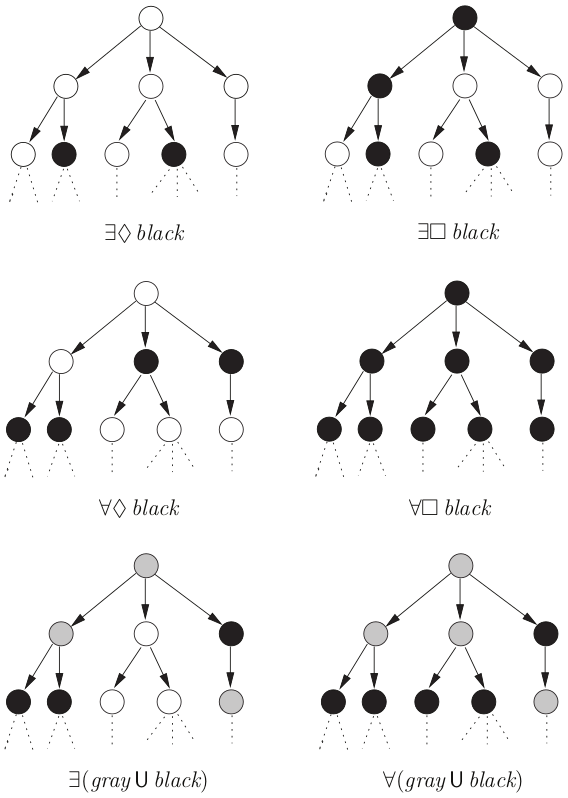
\includegraphics[width=0.8\textwidth]{ctl/imagenes/semanticaCTL.png}
\label{fig:semantica_CTL}
\end{center}
\end{minipage}
\end{figure}


\subsection{Propiedades}
En esta sección se muestran propiedades útiles para poder expresar todas las fórmulas
 de CTL utilizando un conjunto reducido y funcionalmente completo de conectivos.

\begin{itemize}
\item $\exists \lozenge \varphi = \exists (true \cup \varphi) $
\item $\forall \lozenge \varphi = \forall (true \cup \varphi) $
\item $\exists \square \varphi = \lnot \forall \lozenge \lnot \varphi $
\item $\forall \square \varphi = \lnot \exists \lozenge \lnot \varphi $
\item $\forall \bigcirc \varphi = \lnot \exists \bigcirc \lnot \varphi $
\item $\forall \lozenge \varphi = \lnot \exists \square \lnot \varphi $
\end{itemize}

Con estas propiedades es posible expresar cualquier propiedad en CTL mediante
 una fórmula CTL equivalente que sólo contenga el cuantificador existencial.


\subsection{CTL vs LTL}
Tanto CTL como LTL son lenguajes que permiten expresar muchas propiedades para un sistema.
 Pero son lógicas incompatibles entre sí. Esto quiere decir que existen fórmulas de CTL
 para las cuales no hay una equivalente en LTL y viceversa.

\begin{definicion}
Equivalencia entre fórmulas CTL y fórmulas LTL.\\
Una fórmula CTL $\varphi$ y una fórmula LTL $\psi$ son equivalentes si para todo
 sistema de transiciones $TS$:
\[ TS \models \varphi \text{ si y solo si } TS \models \psi \]
\end{definicion}

Un estado satisface una fórmula LTL $\varphi$ cuando todos los caminos a partir de
 este estado satisfacen $\varphi$.
De esto se puede observar que para obtener una fórmula LTL equivalente a una
 fórmula CTL dada basta con eliminar los cuantificacdores universales de la misma.
Más precisamente, dada una fórmula CTL, en caso de que exista un fórmula LTL
 equivalente, esta se obtiene eliminando los cuantificadores tanto universales
 como existenciales de la misma.
 

%\chapter{Implementación del verificador}
%Dado un sistema de transiciones $T$ que modela nuestro sistema, se quiere determinar si todas sus ejecuciones
 cumplen con una propiedad dada $\varphi$.
 
\[ ejecuciones(T) \subseteq \mathcal{L} (\varphi) \]

Este problema se puede ver como determinar si existe una ejecución del sistema que no cumple $\varphi$,
 o dicho de otra forma, que cumple $\lnot \varphi$.

\[ ejecuciones(T) \cap \mathcal{L} (\lnot \varphi) = \emptyset \]

El procedimiento para verificarlo consta de tres pasos. Cada uno de ellos se puede tratar
 de forma individual.

El primer paso es construir un NBA $\mathcal{A}$ que reconozca los malos comportamientos, esto es
 que reconozca las palabras que cumplen con $\lnot \varphi$. Este autómata es útil para encontrar las
 ejecuciones que no cumplen con la propiedad deseada.

A continuación se debe realizar el producto $T \otimes \mathcal{A}$, donde $T$ es el modelo de nuestro sistema
 y $\mathcal{A}$ el autómata obtenido en el paso anterior. De esta forma intersectamos las ejecuciones
 de nuestro sistema con las palabras que no cumplen la propiedad a verificar.

Por último debemos verificar que el lenguaje representado por el autómata resultante es vacío, esto significa
 que no hay ninguna ejecución del sistema que no cumple con la propiedad. En caso de no ser vacío, cualquiera
 de las palabras contenidas en él sirve como contraejemplo.
 %es una ejecución del sitema que no cumple con la propiedad.
 

\subsection{Construcción de un GNBA a partir de una fórmula LTL}

%- Conjuntos elementales
Veremos como construir un GNBA a partir de una fórmula $\varphi$.

Lo primero es calcular el conjunto $clausura( \varphi )$ que se define a continuación.

\begin{definicion}
Clausura. \\
La clausura de una fórmula LTL es el conjunto formado por todas sus subfórmulas y sus negaciones.
\end{definicion}

Ahora se necesita construir los conjuntos elementales con respecto a $clausura( \varphi )$.\\

\begin{definicion}
Conjunto elemental.\\
Sea $B$ un subconjunto de la clausura $\varphi$.
$B$ es un conjunto elemental de $\varphi$ si cumple:
\begin{itemize}
\item es consistente con respecto a la lógica proposicional:
	\begin{itemize}
	\item $\varphi_1 \wedge \varphi_2 \in B \Longleftrightarrow \varphi_1 \in B$ y $\varphi_2 \in B$
	\item $\neg \psi \in B \Longrightarrow \psi \not\in B$
	\item $true \in clausura(\varphi ) \Longrightarrow true \in B$
	\end{itemize}
\item es maximal:
	\begin{itemize}
	\item $\varphi_2 \in B \Longrightarrow \varphi_1 \cup \varphi_2 \in B$
	\item $\varphi_1 \cup \varphi_2 \in B$ y $\varphi_2 \not\in B \Longrightarrow \varphi_1 \in B$
	\end{itemize}
\item es localmente consistente con respecto al operador until:
	\begin{itemize}
	\item $\psi \not\in B \Longrightarrow \neg \psi \in B$
	\end{itemize}
\end{itemize}
\end{definicion}



%- Reglas para construirlos
%figura 5.20


% construccion del gnba - página 278
Una vez definidos los conceptos anteriores se puede comenzar a construir el GNBA para una
fórmula LTL de la siguiente manera:
\begin{enumerate}
\item El conjunto de estado está formado por todos los conjuntos de fórmulas elementales de
 $\varphi$
\item $Q_0 = \{ B \in Q | \varphi \in B \}$ \\
El conjunto de estados iniciales está formado por todos los estados que contienen a $\varphi$
\item $F = \{ F_{\varphi_1 \cup \varphi_2} | \varphi_1 \cup \varphi_2 \in clausura(\varphi) \}$ donde 
$F_{\varphi_1 \cup \varphi_2} = \{ B \in Q | \varphi_1 \cup \varphi_2 \not\in B$ o $ \varphi_2 \in B\}$ \\
es el conjunto de aceptación
\item La relación de trasición $\delta : Q \times 2^{AP} \rightarrow 2^Q$ queda definida por:
\begin{itemize}
\item si $A \neq B \cap AP$ entonces $\delta (B,A) = \phi$
\item si $A = B \cap AP$ entonces $\delta (B,A) = B'$, donde $B'$ es el conjunto elemental de fórmulas
que cumple:
\begin{itemize}
\item[i] para cada $\bigcirc \psi \in clausura(\varphi) : \bigcirc \psi \in B \Leftrightarrow \psi \in B'$ y
\item[ii] para cada $\varphi_1 \cup \varphi_2 \in clausura(\varphi ):$ \\
$\varphi_1 \cup \varphi_2 \in B \Leftrightarrow (\varphi_2 \in B \vee (\varphi_1 \in B \wedge \varphi_1 \cup \varphi_2 \in B'))$
\end{itemize}
\end{itemize}
\end{enumerate}

Con este mecanismo podemos generar un GNBA para cualquier fórmula LTL, asumiendo que estas fórmulas LTL
 contienen únicamente los conectivos $true$, $\lnot$, $\land$, $\bigcirc$ y $\cup$. En caso de que esto
 no se cumpla, se puede generar un GNBA para una fórmula equivalente que utilice sólo estos conectivos
 con las propiedades vistas anteriormente.

\paragraph{Ejemplo.}
Considerando la fórmula $\varphi = a \cup b$.\\
Los conjuntos de fórmulas elementales de $\varphi$ son:
\[
B_1 = \{ a, b, \varphi \}, 
B_2 = \{ \lnot a, b, \varphi \}, 
B_3 = \{ a, \lnot b, \varphi \}, 
B_4 = \{ \lnot a, \lnot b, \lnot \varphi \}, 
B_5 = \{ a, \lnot b, \lnot \varphi \}
\]

Los estados iniciales son los conjuntos $B_i$ tal que $\varphi \in B_i$. $Q_0 = \{ B_1, B_2, B_3 \}$.

El conjunto de conjuntos de aceptación es $F = \{ F_\varphi \}$, donde
\[ F_\varphi = \{ B \in Q | \varphi \in B \vee q \in B \} = \{ B_1, B_2, B_4, B_5 \} \]
El GNBA resultante se muestra en la figura \ref{fig:GNBA_formula}.
\begin{figure}[hbtp]
\begin{minipage}{\textwidth}
\begin{center}
\caption[GNBA para la fórmula $ a \cup b $]%
{GNBA para la fórmula $ a \cup b $ \footnote[1]{Imagen tomada de \cite{katoen}}}
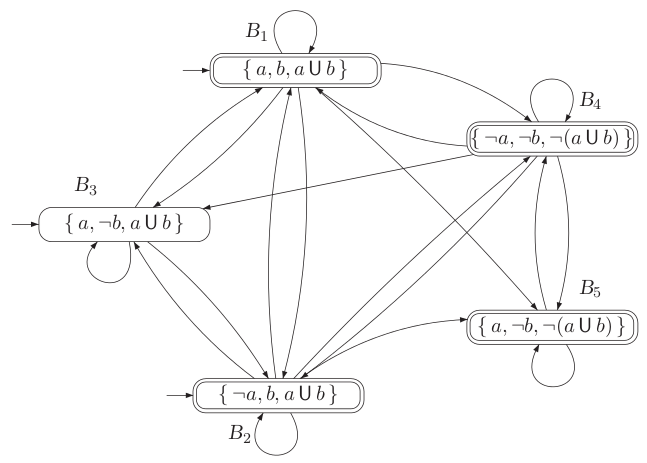
\includegraphics[width=0.8\textwidth]{ltl/imagenes/figura5_22.png}
\label{fig:GNBA_formula}
\end{center}
\end{minipage}
\end{figure}


%Luego se debe determinar si las trazas del sistema de transiciones T no contienen ninguna palabra
% que sea reconocida por A, o sea un mal comportamiento de nuestro sistema.

Una vez obtenido el GNBA para una fórmula $\varphi$ debemos transformar este en un NBA equivalente.
Para esto primero debemos entender la principal dieferencia entre ambos.
Esta radica en su criterio de aceptación. Una palabra es reconocida (o aceptada) por un NBA si esta
pasa infinitas veces por al menos un estado de su conjunto de aceptación. Mientras que una palabra
es reconocida por un GNBA si esta pasa infinitas veces por al menos un estado de cada conjunto de
 aceptación.

Sabiendo esto se puede encontrar un método sencillo para transformar un GNBA en un NBA equivalente.

Sea $\mathcal(G)$ un GNBA y $\mathcal(F) = \{ F_1 , ..., F_k \} $ el conjunto formado por todos sus
 estados de aceptación.
El método consiste en crear $k$ copias de $\mathcal(G)$ tales que cada estado del conjunto $F_i$ está
 conectado con los correspondientes estados en la copia $i + 1$ como se muestra en la
 figura \ref{fig:GNBA_to_NBA}.

%IMAGEN pag 195
\begin{figure}[hbtp]
\begin{minipage}{\textwidth}
\begin{center}
\caption[Generación de un NBA a partir de un GNBA]%
{Generación de un NBA a partir de un GNBA \footnote[1]{Imagen tomada de \cite{katoen}}}
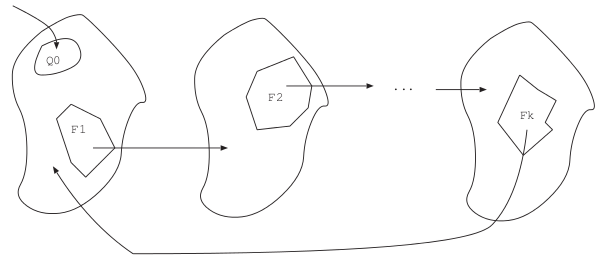
\includegraphics[width=0.8\textwidth]{ltl/imagenes/figura4_20.png}
\label{fig:GNBA_to_NBA}
\end{center}
\end{minipage}
\end{figure}

El conjunto de aceptación del NBA resultante es el conjunto $F_1$ de la copia 1.

De esta forma nos aseguramos de que toda palabra que pase infinitas veces por alguno de los estados
 de $F_1$ pasa infitas veces por al menos un estado de cada conjunto de aceptación de $\mathcal{G}$.



\subsection{Producto}

En segundo lugar se realiza el producto $T \otimes \mathcal{A}$, siendo $\mathcal{A}$ el NBA resultante
 de la parte anterior.

El lenguaje reconocido por el producto de dos autómatas es la intersección de los lenguajes reconocidos
 por cada uno de ellos.

El producto $\mathcal{A} = \mathcal{A}_1 \otimes \mathcal{A}_2 $ queda definido de la siguiente manera
\begin{itemize}
\item El conjunto de estados $Q = Q_1 \times Q_2$ siendo $Q_1$ y $Q_2$ los conjuntos de estados de
 $\mathcal{A}_1$ y $\mathcal{A}_2$ respectivamente.
\item El conjunto de estados iniciles $Q_0 = Q_{0_1} \times Q_{0_2}$ siendo $Q_{0_1}$ y $Q_{0_2}$ los conjuntos
 de estados iniciales de $\mathcal{A}_1$ y $\mathcal{A}_2$ respectivamente.
\item La función de transición $\delta$ cumple
\[  \delta_1(q_1, A) = q'_1 ~~  y ~~ \delta_2(q_2, A) = q'_2 ~~ entonces ~~ \delta((q_1,q_2), A) = (q'_1,q'_2)\]
\item En este proyecto se trabaja con sistemas reactivos, y al estos no tener estados finales, el conjunto de
 aceptación es $F= \{ (q_1,q_2) | q_1 \in F_1 \}$ siendo $F_1$ el conjunto de aceptción de $\mathcal{A}_1$.
\end{itemize}


\subsection{Algoritmo de verificación}
Por último se debe verificar si las trazas del sistema de transiciones $T$ no contienen ninguna palabra
 que sea reconocida por $\mathcal{A}$, o sea un mal comportamiento de nuestro sistema. Esto significa que
 ninguna ejecución de $T$ es reconocida por el autómata $\mathcal{A}$.

Lo anterior es equivalente a controlar que $T \otimes \mathcal{A} \models \lozenge \box \lnot F$
 siendo $F$ un estado de aceptación.
Esto se logra verificando si existe algún estado de aceptación alcanzable y que al mismo tiempo pertenezca
 a un ciclo.
 


\chapter{Conclusiones}
%
Intro .... que se hizo, puntos a favor, etc..

\section{Trabajo futuro}

El principal trabajo futuro sería ...

Sería muy útil contar con una funcionalidad de depuración, la cuál
mostrara dependiendo del tiempo los valores de cada fuente de eventos.

Una opción es comunicar mediante el puerto serial el valor de cada
señal al cambiar, y mostrarlo en una interfaz web como la que provee
RXMarbles (ver \cite{rxmarbles}). 
El lenguaje Elm provee de una herramienta que permite viajar en el 
tiempo, modificar y mostrar la ejecución de un programa, en nuestro
caso no sería posible modificar lo que el robot físico realiza, pero
si sería útil ver en la línea de tiempo que valores tomaron sus
señales. (ver \cite{elmdebug})



% Bibliografia
\cleardoublepage
\addcontentsline{toc}{chapter}{Bibliografía}
\begin{thebibliography}{99}
\bibitem{katoen} \emph{Principles of Model Checking}.\\
 Christel Baier y Joost-Pieter Katoen.\\
 The MIT Press, 2008.

% http://conal.net/papers/frp.html
%@InProceedings{ElliottHudak97:Fran,
%  title        = {Functional Reactive Animation},
%  url          = {http://conal.net/papers/icfp97/},
%  author       = "Conal Elliott and Paul Hudak",
%  booktitle    = "International Conference on Functional Programming",
%  year         = 1997
%}

% Yampa, Arrows and Robots.

%@InProceedings{Peterson99:LambdaInMotion,
%  author       = {John Peterson and Paul Hudak and Conal Elliott},
%  title        = {Lambda in Motion: Controlling Robots with {Haskell}},
%  url          = {http://haskell.org/frob/padl99/padl99.ps},
%  booktitle    = {Practical Aspects of Declarative Languages},
%  year         = 1999
%}
% http://cs.brown.edu/research/pubs/techreports/reports/CS-03-20.html

% Informal pero ayudo:
% https://gist.github.com/staltz/868e7e9bc2a7b8c1f754
%
% Rx, Bacon.js, 
%
% Para debug muy bueno: (con RX es este)
% https://github.com/jaredly/rxvision
% http://lambdor.net/?p=44

% Elm Creator:
% Evan Czaplicky "Controlling Time and Space. https://www.youtube.com/watch?v=Agu6jipKfYw a video can be a reference? "
% elm-lang.org/papers/concurrent-frp.pdf (evan czaplicky thesis)
% SEGUIR CON:::j
% https://vimeo.com/77164337

\bibitem{python} Sitio web de \emph{Python 2.7}:\\
 \url{http://docs.python.org/2/}\\
 Último acceso: 31/10/2013.

\bibitem{gml} Sitio web de \emph{GraphML File Format}:\\
 \url{http://graphml.graphdrawing.org/}\\
 Último acceso: 31/10/2013.

\end{thebibliography}


% Apendices
\appendix
\cleardoublepage
\addappheadtotoc
\appendixpage

%\chapter{Manual de usuario}
%

  Para utilizar el compilador, dado un archivo \textit{Ejemplo.willie}, se
ejecuta:

\begin{Verbatim}
> williec < Ejemplo.willie > Ejemplo.alf
\end{Verbatim}



El código de la máquina virtual está en el directorio
  /src/alfvm, para compilarlo se ejecuta:
\begin{verbatim}
  > cd src/alfvm
  > make
\end{verbatim}



%
%\chapter{Archivos \textit{GraphML}}
%Como se mencionó anteriormente se utilizó el formato de archivo \textit{GraphML} para
 representar los sistemas de transiciones.
Los estados son representados por el elemento \texttt{node} mientras que las transiciones
 son representadas por el elemento \texttt{edge}.

El formato \textit{GraphML} no establece como representar las etiquetas tanto en los nodos
 como en las aristas.
Para esto existe el atributo \texttt{data}, que proporciona flexibilidad
 para agregar atributos no contemplados por el formato.
Esto tiene un desventaja, y es que los atributos no contemplados por el formato no se
 representan de forma estándar, y por lo tanto su representación depende del editor
 utilizado.
En este caso el editor utilizado es \textit{yEd}.

Para los estados se guarda la siguiente información:
\begin{itemize}
\item Identificador

Este valor se guarda en el atributo \texttt{id} de cada nodo.
Es el identificador del estado, por lo que debe ser único.

Cuando se genera un sistema de transiciones mediante el verificador este genera los identificadores
 de cada estado automáticamente.

\item Proposiciones

Representan el conjunto de las proposiciones válidas en cada estado.

Se guardan en el atributo \texttt{y:NodeLabel}.
Este atributo es se encuentra dentro del atributo \texttt{data}, ya que no se encuentra
 especificado en el formato.

En caso de haber varias proposiciones, estas deben estar separadas por comas.

\end{itemize}

Además de esta información se debe indicar cuales son los estados iniciales.

Para las transiciones se debe guardar la siguiente información:
\begin{itemize}
\item Origen

Representa el estado de origen de la transición. Se guarda en el atributo \texttt{source}.

\item Destino

Representa el estado de destino de la transición. Se guarda en el atributo \texttt{target}.

\item Acción

Representa la acción que corresponde al cambio de estado.

Se guardan en el atributo \texttt{y:EdgeLabel}.

Este atributo es se encuentra dentro del atributo \texttt{data}, ya que no se encuentra
 especificado en el formato.

\end{itemize}

El parser de \textit{GraphML} a sistemas de transiciones se encuentra implementado en
 el objeto \texttt{ParserGraphML} del paquete \textit{Sistemas de transiciones}.

Como se mencionó anteriormente hay atributos que no están especificados en el formato y
 por lo tanto su interpretación depende del editor utilizado. Estos atributos son especificados
 en el parser mediante sub clases.
En este caso se utiliza el \textit{yEd Graph Editor}, para el cual fue implementado el objeto
 \texttt{ParserGraphML\_yEd}.
Este objeto es un parser de \textit{GraphML} que además interpreta la información dentro del
 atributo \texttt{data} como las etiquetas de los estados y transiciones.

A continuación se muestra un ejemplo de un sistema de transiciones y su correspondiente
 representación en \textit{GraphML}.

\paragraph{Ejemplo de sistema de transiciones en \textit{GraphML}} 





% Termina el documento
\end{document}
